\documentclass[12pt]{article}
\usepackage[12pt]{moresize}

\usepackage{amsmath}
\usepackage{amssymb}

\usepackage{graphicx}
\usepackage{subcaption}

\usepackage{algorithm}
\usepackage{algpseudocode}
\usepackage{alltt}

\usepackage{multicol}

\usepackage[margin=1in]{geometry}

%\usepackage{hyperref}
%\usepackage[latin1]{inputenc}
%\usepackage{listings}
%\usepackage{scrextend}
%\usepackage{changepage} %Adjustwidth


\newenvironment{PTMono}{\fontfamily{PTMono-TLF}\selectfont}{\par}


\title{ComS 363\\Homework 4}
\author{Sean Gordon}
\date{April 24, 2020}

\begin{document}
\maketitle


\hrulefill \\



\noindent 1)\\
\indent \indent With 4000 B per page and 400 B per tuple, each page can contain 10 tuples.\\
\indent \indent This leaves R to take 1000 pages, and S to take 200 pages.\\\\
\indent (a) Testing R as outer:\\
\indent \indent Need 1000 I/Os to read outer, and 4000 to join\\
\indent \indent Total = 1000 + 4000 = 5000 I/Os\\\\
\indent \indent Testing S as outer:\\
\indent \indent Need 200 I/Os to read outer, and 4000 to join\\
\indent \indent Total = 200 + 4000 = 4200 I/Os\\\\
\indent \indent 4200 $<$ 5000 $\Rightarrow$ Using S as outer, cost is 4200 I/Os\\\\
\indent \indent Buffer should contain the entirety of the smaller relation (S), plus the output and \\
\indent \indent the inner relation size.\\
\indent \indent Thus buffer must be of size 200 + 1 + 1 = 202 pages\\


\indent (b) Partition:\\
\indent \indent 2 * R + 2 * S $\Rightarrow$ 2(1000) + 2(200) = 2400 I/Os\\\\
\indent \indent Probing:\\
\indent \indent Buffer (52) must be $\ge$ (fudge)(N)/(Mem - 1) $\Rightarrow$ (1.1)(1000)/(52 - 1) = 21.5 \checkmark \\
\indent \indent I/O for this section is then 1000 + 200 = 1200\\\\
\indent \indent Total I/O cost = 2400 + 1200 = 3600 I/Os\\

\pagebreak

\indent (c) Sorting:\\
\indent \indent Cost for R = 2(2 * 1000) = 4000 \indent \indent Cost for S = 2(2 * 200) = 800\\\\
\indent \indent Merging:\\
\indent \indent Cost = 1000 + 200 = 1200 I/Os\\\\
\indent \indent Total = 4000 + 800 + 1200 = 6000 I/Os\\


\hrulefill\\


\noindent 2)\\
\indent \indent (a) {\large $\Pi_{sname}((\sigma_{bname=''Odyssey''}(Reserve \bowtie Boats)) \bowtie Sailors )$} 
\begin{figure}[h!]
  \centering
  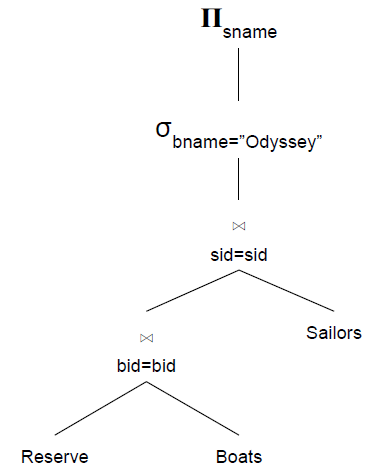
\includegraphics[scale=.6]{Q2a.PNG}
\end{figure}\\


\indent \indent (b) {\large $\Pi_{sname}(\sigma_{day=''05/15/2020''}(Sailors \bowtie Reserve))$} 
\begin{figure}[h!]
  \centering
  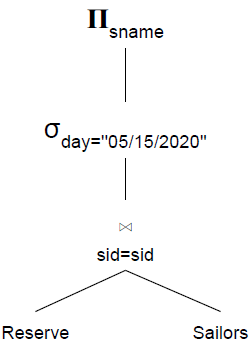
\includegraphics[scale=.6]{Q2b.PNG}
\end{figure}

\pagebreak


\indent \indent (c) {\large $\Pi_{sname}(Sailors - (Sailors \bowtie Reserve)))$} 
\begin{figure}[h!]
  \centering
  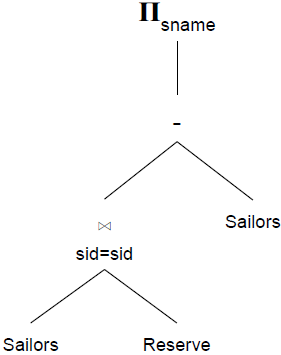
\includegraphics[scale=.5]{Q2c.PNG}
\end{figure}



\end{document}
















